\documentclass[12pt,a4paper]{report} %Formato y formas principales
\usepackage[spanish]{babel} %Establecer idioma
\usepackage{graphicx} %Para añadir imágenes
\usepackage{fancyhdr} %Para establecer mi propio encabezado y pie de página
\usepackage[left=3cm,right=3cm,top=2.5cm,bottom=2.5cm,headsep=1cm]{geometry} % Mis márgenes
%\setlength{\headheight}{14.0pt} %Ajusta el tamaño del encabezado
%\linespread{1.5} % Espaciado de 1.5 (1 es el espaciado estándar)
\setlength{\parindent}{0pt} %Ajusta la sangría a 0 para que no haya
\usepackage{amsmath} %Para ecuaciones\usepackage{amsmath}
\usepackage{multicol}
%\usepackage{refcheck} %Para que aparezca el nombre que le doy a la referencia
\usepackage{comment} %Para comentar varias lineas
\usepackage{lipsum} %Para hacer textos de ejemplo para pruebas

\usepackage{caption} %Para crear mi formato "boldformat" que pone lo primero en negrita
\DeclareCaptionFormat{boldformat}{\textbf{#1} #2 #3}
\captionsetup[figure]{format=boldformat} %Le asigno el formato al de las figuras

\usepackage{hyperref} %Para que haya hipervínculos
\hypersetup{
	colorlinks=true, %Para que los hipervínculos sean de color y no con caja roja
	linkcolor=black,
	urlcolor=black,
	citecolor=black,
}

\makeatletter %Mi propio comando para establecer las referencias de figuras y ecuaciones
\newcommand{\figureref}[1]{\hyperref[#1]{\textcolor{blue}{\textit{Figura~\ref*{#1}}}}}
\newcommand{\equationref}[1]{\hyperref[#1]{\textcolor{blue}{\textit{Ecuación~\ref*{#1}}}}}
\makeatother

\usepackage{makeidx} %Para hacer el indice
\makeindex
\usepackage{tocloft} %Para configurar el índice
\renewcommand{\cftchapleader}{\cftdotfill{\cftdotsep}} %Línea puntos índice
\setlength{\cftbeforetoctitleskip}{-1cm} % Ajusta el margen superior del índice

\usepackage[T1]{fontenc} %Para cambiar la letra y el tamaño
\usepackage[scaled]{uarial}
\renewcommand*\familydefault{\sfdefault}


\usepackage{titlesec} %Para cambiar mi formato de chapter
\titleformat{\chapter}[display]
{\normalfont\huge\bfseries}{\chaptertitlename\ \thechapter}{20pt}{\LARGE}
\titlespacing*{\chapter}{0pt}{-1.5cm}{40pt}

\pagestyle{fancy}
\fancyhf{}
\fancyhead[L]{\fontsize{12}{14}\selectfont\leftmark}  % Número de página a 
\fancyhead[R]{\fontsize{12}{14}\selectfont\thepage}  % Número de página 
\fancyfoot[R]{\fontsize{12}{14}\selectfont Sevilla, Julio de 2023}  % 


\begin{document}
	
	\begin{titlepage}
		\centering
		\hspace*{-1.5cm}\begin{tabular}{@{}l@{}}
			
\includegraphics[width=3cm]{b.png} % Logo 1 (esquina superior izquierda)
		\end{tabular}
		\hfill
		\begin{tabular}{c}
			\LARGE\textbf{Universidad de Sevilla} \\ [0.5cm] % Nombre de la universidad
			\LARGE\textbf{Escuela Politécnica Superior} % Otra frase dentro de la misma caja
		\end{tabular}%
		\hfill
		\begin{tabular}{@{}r@{}}
			
\includegraphics[width=3cm]{a.png} % Logo 2 (esquina superior derecha)
		\end{tabular}\hspace*{-1.5cm}
		
		\vspace{1.5cm}
		
		\begin{center}
			\Large\textmd{Trabajo Fin de Grado} \\ [0.2cm] % Título 
			\Large\textmd{Ingeniería Electrónica Industrial}
		\end{center}
		
		\vspace{2cm}
		
		\begin{center}
			\LARGE\textsl{La caracterización integral de las semiaplicaciones de Poincaré y su aplicación a circuitos electrónicos: El Memristor}
		\end{center}
		
		\vspace{7cm}
		
		\raggedright
		\large\textbf{Autor:} Sergio R. Durán Martín \\ [0.5cm]
		\large\textbf{Tutor:} Dr. Victoriano Carmona Centeno \\ [0.5cm]
		\large\textbf{Departamento:} Matemática Aplicada II
	\end{titlepage}
	
	\clearpage
	\null
	\thispagestyle{empty}
	\newpage

\begin{center}
	\LARGE\textbf{Resumen}
\end{center}
\begin{minipage}{\textwidth}
	\lipsum[1]
	
	\vspace{0.5cm}
	\noindent \textbf{Palabras clave:} robótica educativa, robot modular, STM32, FreeRTOS, interfaz gráfica, impresión 3D.
\end{minipage}

\vspace{1cm}

\begin{center}
	\LARGE\textbf{Abstract}
\end{center}
\begin{minipage}{\textwidth}
	\lipsum[2]
	
	\vspace{0.5cm}
	\noindent \textbf{Keywords:} educational robotics, modular robot, STM32, FreeRTOS, graphic interface, 3D printing.
\end{minipage}
\newpage
	
\tableofcontents
	\chapter{Introducción}
	Contenido del capítulo de introducción. Contenido del capítulo 1.
	
	\chapter{Descripción del Circuito}
	El circuito que se ha estudiado es un oscilador con resistencia negativa al que se le ha añadido un componente muy interesante y que está siendo muy estudiado en estos últimos tiempos, el memristor, ver \figureref{fig:-RLCM}.
	
	\begin{figure}[h]
		\centering
		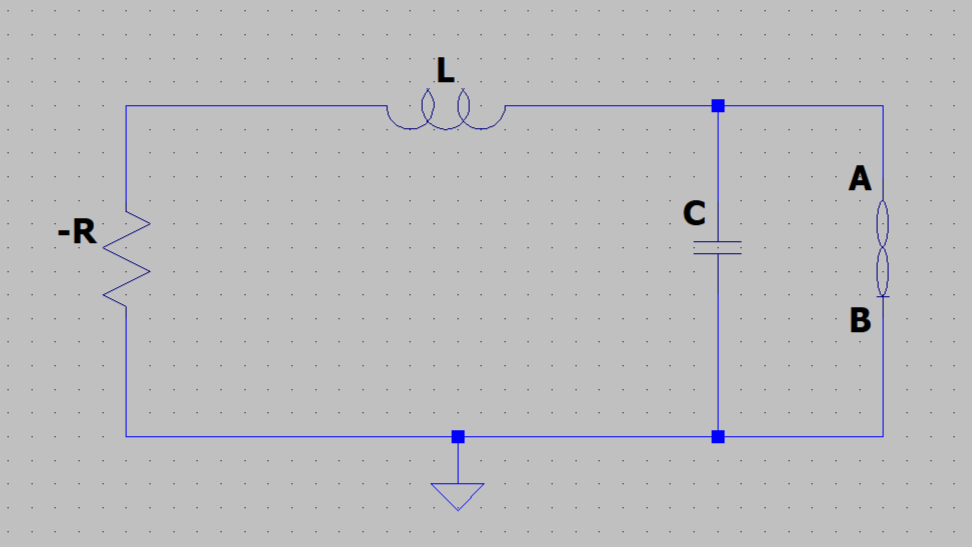
\includegraphics[width=0.7\textwidth]{-RLCM.png}
		\caption{Oscilador RLC con R negativa y Memristor}
		\label{fig:-RLCM}
	\end{figure}
	
	Como se puede ver no existe una fuente de señal en el circuito y esto se debe a que el análisis hecho busca encontrar una oscilación periódica tan solo proporcionando condiciones iniciales a la bobina y el condensador, esto gracias al comportamiento de la resistencia negativa y del memristor los cuales se especifican mas adelante.\\[0.5cm]
	La forma de imponer las condiciones iniciales serían las clásicas, usando fuentes de intensidad en serie y tensión en paralelo con interruptores que se abren en $t\,=\,0(s)$ para la bobina y el condensador respectivamente. Esta parte no se va a detallar más en profundidad puesto que en este trabajo no hay implementación real del circuito, los motivos se detallan en el CAPITULO X.
	\newpage
	\section{Resistencia negativa}
	Uno de los componentes del circuito es la resistencia negativa la cual se puede construir con lo que se llama un \emph{Convertidor de Impedancia Negativa (NIC)}. Un NIC es un circuito activo, es decir, en lugar de disipar energía como una resistencia convencional, puede proporcionar energía a un circuito, ver \figureref{fig:NIC}. En términos prácticos, un NIC puede ser utilizado para compensar la resistencia de carga de un sistema, mejorar la eficiencia de la transferencia de energía o realizar otras funciones específicas en circuitos eléctricos o electrónicos. En los circuitos osciladores, el NIC desempeña un papel importante en el mantenimiento, estabilización, frecuencia y calidad de la oscilación.
	 
	\begin{figure}[h]
		\centering
		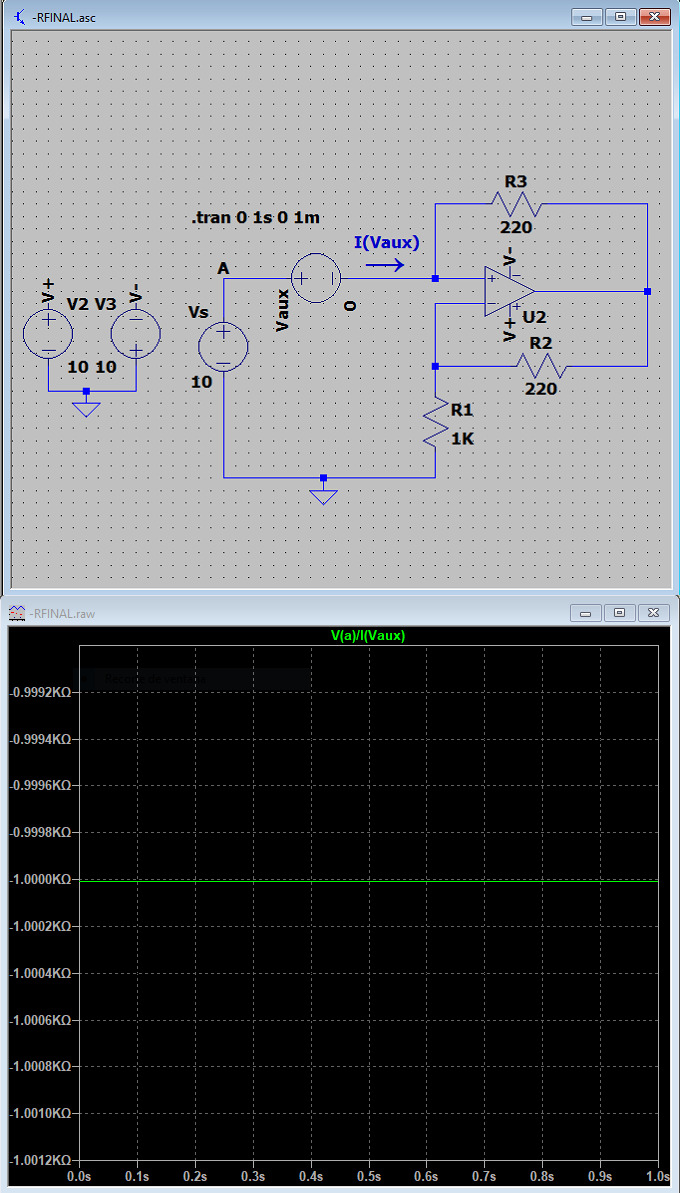
\includegraphics[width=0.65\textwidth]{NIC_B.jpg}
		\caption{Convertidor de Impedancia Negativa de -1000 Ohmios}
		\label{fig:NIC}
	\end{figure}
	
	\newpage
	
	Una de las maneras de realizarlo es usando un amplificador operacional y 3 resistencias en la configuración que se ve en la \figureref{fig:NIC} de esta manera si elegimos $R_2=R_3$ la resistencia $R_1$ es la que determinaría el valor de resistencia negativa, esta es la demostración:
	
	\begin{center}
	\begin{multicols}{2}
		\centering
		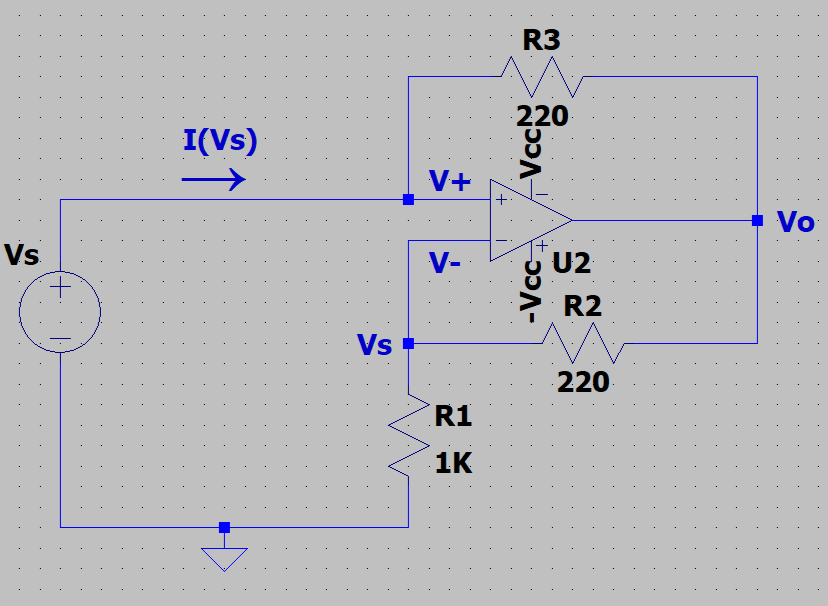
\includegraphics[width=\columnwidth]{demotracion_NIC.png}
		\captionof{figure}{Parámetros circuito NIC }
		\label{fig:Param_NIC}
	
		\columnbreak
		
		Consideraciones para el cálculo del circuito de la \figureref{fig:Param_NIC} con Amplificadores Operacionales:\\
		\begin{equation}
			V_+\,=\,V_-
			\label{eq:NIC1}
		\end{equation}
		\begin{equation}
			I_+\,=\,I_-\,=\,0\,(A)
			\label{eq:NIC2}
		\end{equation}
	\end{multicols}
	\end{center}
	
	Teniendo en cuenta la \equationref{eq:NIC1} se puede ver que la tensión $V_S$ cae sobre $R_1$ y se puede relacionar con $V_O$ mediante un divisor de tensión:
	
	\begin{equation}
		V_S\,=\,V_O\,\frac{R_1}{R_1 + R_2}\:\longrightarrow\:V_O\,=\,V_S\,\frac{R_1 + R_2}{R_1}
		\label{eq:NIC3}
	\end{equation}\smallskip
	
	Teniendo en cuenta la \equationref{eq:NIC2} se puede ver que la intensidad $I(V_S)$ es la misma que pasa por la $R_3$, por ello se puede deducir:
	
	\begin{equation}
		I(V_S)\,=\,\frac{V_S - V_O}{R_3}
		\label{eq:NIC4}
	\end{equation}\smallskip
	
	Sustituyendo la \equationref{eq:NIC3} en \equationref{eq:NIC4} y trabajando la expresión se llega a:
	
	\begin{equation}
		I(V_S)\,=V_S\,\frac{-R_2}{R_1 \cdot R_3}
		\label{eq:NIC5}
	\end{equation}\smallskip
	
	Si dividimos $V_S$ entre $I(V_S)$ (\equationref{eq:NIC5}) para obtener la impedancia de entrada:
	
	\begin{equation}
		\frac{V_S}{I(V_S)}\,=\,Z_{IN}\,=\,\frac{V_S}{V_S\,\frac{-R_2}{R_1 \cdot R_3}}\,=\,-R_1\,\frac{R_3}{R_2}
		\label{eq:NIC6}
	\end{equation}\smallskip
	
	Si elegimos $R_3\,=\,R_2$ en la \equationref{eq:NIC6} obtenemos:
	
	\begin{equation}
		Z_{IN}\,=\,-R_1
		\label{eq:NIC7}
	\end{equation}\smallskip
	
	\newpage
	\section{Memristor}
	esto es texto de la siguiente hoja
	\newpage
	\section{Variables de estado}
	esto es texto de la siguiente hoja
	\newpage
	\section{Superficies invariantes}
	esto es texto de la siguiente hoja
	
	\chapter{Sistemas Lineales a Trozos Bizonales}
	Contenido del capítulo 3.
	\newpage
	\section{Sistemas lineales planos}
	esto es texto de la siguiente hoja
	\newpage
	\section{Sistemas lineales a trozos bizonales}
	esto es texto de la siguiente hoja
	
	\chapter{Semiaplicaciones de Poincaré}
	Contenido del capítulo 4.
	\newpage
	esto es texto de la siguiente hoja
	
	\chapter{Bifurcación Foco-Centro-Ciclo Límite}
	Contenido del capítulo 5.
	\newpage
	esto es texto de la siguiente hoja
	
	\chapter{Oscilación Peródica en el circuito}
	Contenido del capítulo 6.
	\newpage
	esto es texto de la siguiente hoja
	
	\chapter{TÍTULO CAPÍTULO 7}
	Contenido del capítulo 7.
	\newpage
	esto es texto de la siguiente hoja
	
	\chapter{TÍTULO CAPÍTULO 8}
	Contenido del capítulo 8.
	\newpage
	esto es texto de la siguiente hoja
	
	\chapter*{Conclusiones}
	Contenido del capítulo de conclusiones.
	\newpage
	esto es texto de la siguiente hoja
	
	\begin{comment}
	\chapter{Introducción}
	\begin{equation}
		\label{EcuLambda}
		y^2=3
	\end{equation}
	hola mundo prueba script prueba branch de funcion $f$ \eqref{EcuLambda} en $[2\pi]$
	\newpage
	holaaa
	\newpage
	asldkakdlkad prueba python para commit cambio
	\newpage
	\section{introa}
	holaaa
	\newpage
	\subsection{introb}
	segundo cambio tercera prueba python siguiente prueba para ver fuente
	\end{comment}
\end{document}
